\documentclass[10pt,conference]{IEEEtran}
\IEEEoverridecommandlockouts

\usepackage[utf8]{inputenc}
\usepackage[T1]{fontenc}
\renewcommand{\ttdefault}{cmtt}
\usepackage{amsmath}
\usepackage{booktabs}
\usepackage{graphicx}
\usepackage{url}
\usepackage{array}

\graphicspath{{../figures/}{figures/}}

\title{Dependency-Aware Exposure and Augmentation Sequencing for SaaS Presales: The APEX-II Framework}

\author{\IEEEauthorblockN{Akash Anipakalu Giridhar}}

\begin{document}
\maketitle

\begin{abstract}
Occupation-level AI exposure indices score a job as an independent weighted sum of task exposures. This paper shows that assumption is wrong for SaaS presales engineering, and that correcting it produces a practical instrument for planning AI adoption. Building on the first AI Presales Exposure Index (APEX-I), we introduce APEX-II, implemented as STAM, a Segmented, Task-coupled, Adoption and Market model of role survival. APEX-II makes two contributions that do not exist in prior exposure work. First, the Exposure Propagation Multiplier (EPM) measures how much an independent-task score understates true role exposure once within-role task dependencies are modeled. For the Enterprise presales motion the EPM is 1.36, meaning an occupation-level score understates exposure by roughly 36 percent, while the more parallel SMB motion has an EPM of 1.00. Second, the Augmentation Sequencing Policy (ASP) turns the dependency structure into a deployment rule: automate low criticality and low propagation tasks first, and defer discovery and proof-of-concept ownership. Sequenced rollout preserves 1.81 points of Enterprise role survival relative to a naive automatability-first rollout, and this benefit is four times larger in Enterprise than in SMB. We report the full model honestly. It separates strongly from APEX-I in mechanism, it shifts final Role Survival Index from 0.822 under the additive APEX-I baseline to 0.747, and it exposes a real negative result: adding a coarse public-employment calibration layer increased holdout error by 60 percent rather than reducing it. APEX-II is therefore best used as a diagnostic and planning instrument for presales leaders, not as a labor-market forecast.
\end{abstract}

\begin{IEEEkeywords}
AI exposure, presales engineering, sales engineering, task dependency, augmentation sequencing, workforce simulation, SaaS
\end{IEEEkeywords}

\section{Introduction}
SaaS presales engineering is a useful stress test for AI labor exposure modeling because the role sits between codifiable technical production and relationship dependent judgment. A presales engineer writes technical responses, prepares demonstrations, translates ambiguous buyer needs into product narratives, coordinates proofs of concept, handles objections, and builds internal champions. Some of these activities look highly exposed to generative AI. RFP response, first draft demo scripting, call summarization, competitive comparison, and knowledge base retrieval are increasingly within the capability envelope of current language model systems \cite{eloundou2023gpts}. Other activities remain more resistant. Executive discovery, political mapping, trust repair after a failed evaluation, champion development, and high stakes solution positioning depend on context, organizational memory, and credibility that a prompt template cannot reproduce.

APEX-I made this problem measurable. It introduced a Role Survival Index, RSI, for the SaaS presales engineer and used a parametric simulation to compare augmentation and replacement conditions. That first model was intentionally simple. It treated the role as a weighted portfolio of tasks, applied AI adoption assumptions, and reported survival under six conditions ranging from an AI free counterfactual to full AI replacement. The simplicity exposed the shape of the problem, but it also left six limitations. APEX-I did not distinguish Enterprise and SMB sales motions. It relied on expert priors rather than empirical calibration. It had no explicit subtask mechanism test. It disclosed that the market value component was coupled weakly and after the fact rather than inside the survival computation. It used only three seeds. It mapped scenarios informally rather than to external adoption bands.

This paper is Part 2. Its central claim is not merely that presales can be scored, but that presales cannot be scored correctly with the independent task assumption that every existing exposure index uses. Occupation level indices such as the AI Occupational Exposure measure \cite{felten2021occupational} and task level exposure estimates \cite{eloundou2023gpts} treat the tasks of a role as separable and add them up. Presales tasks are not separable. Discovery quality determines demonstration relevance. Demonstration success determines proof-of-concept scope. Champion strength determines whether objections are survivable. When AI absorbs an upstream task, the human value of the downstream tasks changes. An index that ignores this dependency will mis-state both the level and the segment pattern of exposure.

We make three contributions. First, we introduce the Exposure Propagation Multiplier, EPM, a single interpretable number that quantifies how much an independent task score understates role exposure once task dependencies are modeled. Second, we introduce the Augmentation Sequencing Policy, ASP, a deployment rule that uses the dependency structure to order AI rollout so that role survival is preserved during the transition. Third, we deliver APEX-II, a deal-size stratified, subtask level, market coupled simulation that operationalizes these ideas, is reproducible from a single script, and reports its own negative results rather than hiding them. The EPM and ASP are the inventions. APEX-II is the instrument that produces them and lets a presales organization run them on its own task mix.

\section{Related Work}
\subsection{Task Based Automation and Labor Exposure}
Task based labor economics motivates the move from occupation labels to work activity analysis. Technology does not automate an occupation uniformly, it automates tasks, and it also reinstates labor by creating new tasks \cite{acemoglu2019automation}. If a role combines tasks that differ in codifiability, social context, and tacit knowledge, a single exposure score is likely to mislead. Presales is exactly such a role. RFP response and demo scripting are relatively structured. Discovery, champion development, and objection handling are less structured and more socially embedded.

Occupation level AI exposure indices provide useful external comparators but operate at a granularity that is too coarse for presales. The AI Occupational Exposure dataset scores occupations, industries, and geographies \cite{felten2021occupational}, and task level estimates find that a large share of work activities across the economy are exposed to large language models \cite{eloundou2023gpts}. In both, Sales Engineers appear as one occupational category rather than a structured bundle of discovery, demonstration, proof-of-concept, RFP, objection, and champion development work. Firm level exposure measurement built from unstructured text shows that exposure constructs can be made specific and measurable at a finer unit than the occupation \cite{sautner2023firmlevel}. APEX-II applies that spirit inside a single role, and adds the dependency structure that a flat weighted sum cannot represent.

\subsection{Automation and Augmentation}
The automation augmentation paradox is directly relevant to presales. Automation can remove tasks, but it can also raise the value of the tasks that remain \cite{raisch2021artificial}. If AI drafts standard proposals, presales engineers may spend less time on clerical work and more on solution strategy. If AI makes credible demos and technical answers nearly free, organizations may cut human presales headcount for standardized segments. Deployed generative AI systems show real and uneven productivity gains across workers and tasks \cite{brynjolfsson2023generative}, and firm level evidence shows that AI adoption itself is uneven and concentrated \cite{mcelheran2024adoption}. The unresolved question is whether these gains raise the leverage of presales engineers or reduce the number needed per unit of revenue. APEX-II does not assume an answer. It evaluates survival trajectories under scenario conditions and asks where in the task graph augmentation is safe.

\subsection{Presales, Deal Size, and Superstar Dynamics}
The presales engineer is a technical and commercial translator whose value comes from reducing buyer uncertainty, through artifacts such as demos, RFPs, and proof-of-concept plans, and through interaction such as discovery, objection handling, and champion enablement. Deal size shapes this work. Enterprise deals involve multiple stakeholders, security review, integration constraints, procurement friction, and executive sponsorship. SMB deals are more standardized and more amenable to product led evaluation. The same AI capability can therefore have different survival consequences across deal sizes, which connects to broader evidence that technology can concentrate output in a few firms and reshape labor shares \cite{autor2020fall}. APEX-II captures deal size through segment specific dependency structure rather than by assigning Enterprise a blanket resilience bonus.

\section{Method: STAM}
\subsection{Problem Formulation}
Let segment $s \in \{\mathrm{Enterprise}, \mathrm{SMB}\}$, condition $c$, task $k \in \{1,\ldots,6\}$, seed $r$, and quarter $t$. The target is a role survival score $RSI_{s,c,r,t} \in [0,1]$. Higher RSI means more of the presales role remains human anchored. The six tasks are discovery, technical demonstration, proof-of-concept coordination, RFP response, objection handling, and champion development. Each task $k$ has an automation susceptibility $\alpha_k$, the fraction absorbable by AI under adoption pressure, and a role criticality $\beta_k$, the contribution of the task to role survival value, with $\sum_k \beta_k = 1$.

The base weights are expert priors triangulated from two public anchors, the task exposure logic of \cite{eloundou2023gpts} and the occupational exposure structure of \cite{felten2021occupational}, then adjusted for the presales workflow. Structured, template heavy tasks receive high $\alpha$ and lower $\beta$. Relationship anchored tasks receive low $\alpha$ and are protected by dependency structure rather than by weight alone. Table \ref{tab:weights} lists the base configuration. These are priors, not fitted values, and the calibration experiment in Section \ref{sec:calib} tests what happens when a public data anchor is added.

\begin{table}[t]
\caption{Base task configuration. Automation susceptibility $\alpha$ and role criticality $\beta$ are expert priors anchored to public task and occupational exposure sources, not fitted parameters.}
\centering
\begin{tabular}{lrr}
\toprule
Task & $\alpha$ (automatability) & $\beta$ (criticality) \\
\midrule
Discovery & 0.35 & 0.20 \\
Technical demonstration & 0.55 & 0.18 \\
Proof-of-concept coordination & 0.25 & 0.22 \\
RFP response & 0.70 & 0.12 \\
Objection handling & 0.30 & 0.13 \\
Champion development & 0.15 & 0.15 \\
\bottomrule
\end{tabular}
\label{tab:weights}
\end{table}

Subtask survival uses a sigmoid normalized survival model. For task exposure $E_{s,c,k,t}$,
\begin{equation}
RSI_{s,c,k,t}=\sigma(\kappa(\theta - E_{s,c,k,t})),
\end{equation}
where $\sigma$ is the logistic function, $\theta$ the survival midpoint, and $\kappa$ the sharpness. Aggregate role survival is
\begin{equation}
RSI_{s,c,t}=\sum_k \beta_{k} RSI_{s,c,k,t}.
\end{equation}
The extension over APEX-I is the construction of $E_{s,c,k,t}$, which now carries adoption dynamics, dependency propagation, and calibration scaling.

\subsection{Scenario Adoption Curves}
Each condition has an adoption trajectory rather than a static value. A logistic curve maps quarter $t$ to condition intensity,
\begin{equation}
A_c(t)=A^{max}_c(1+\exp[-\rho_c(t-m_c)])^{-1}.
\end{equation}
AFC is an AI free counterfactual, CAB is the current copilot baseline, C24 is a conservative 2024 baseline, PAR is partial automation of structured work, HAO is high adoption with human override, and FAR is full replacement pressure. Conditions are grouped into conservative, baseline, and accelerated bands. They are scenario levers used to test sensitivity, not point forecasts.

\subsection{Dependency Propagation and the EPM}
Presales tasks form a directed acyclic graph $G_s$ that differs by segment. Enterprise uses a serial, dependency rich topology in which discovery feeds demonstration, objection handling, and champion development, and demonstration feeds proof-of-concept and RFP. SMB uses a parallel topology with negligible coupling. Propagated exposure is
\begin{equation}
\tilde{\alpha}_{s,c,k,t} = \alpha_{k} A_c(t) + \lambda \sum_j G_{s,jk}\,\alpha_{j} A_c(t),
\end{equation}
clipped to $[0,1]$, with propagation strength $\lambda = 0.30$.

The first invention follows directly. Define independent role exposure as $\sum_k \beta_k \alpha_k A$ and dependency-aware role exposure as $\sum_k \beta_k \tilde{\alpha}_k$. The Exposure Propagation Multiplier is their ratio at saturating adoption,
\begin{equation}
\mathrm{EPM}_s = \frac{\sum_k \beta_k \tilde{\alpha}_{s,k}}{\sum_k \beta_k \alpha_k}.
\end{equation}
$\mathrm{EPM}_s = 1$ when tasks are independent. $\mathrm{EPM}_s > 1$ means an occupation level or independent task score understates the true role exposure. In the reported run the Enterprise EPM is 1.36 and the SMB EPM is 1.00. An occupation level index therefore understates Enterprise presales exposure by about 36 percent, and understates it more in the exact segment that firms assume is safest.

\subsection{Augmentation Sequencing Policy}
The second invention converts the dependency structure into a deployment rule. Define the role collapse contribution of automating task $k$ as its direct criticality plus the propagated criticality of its downstream neighbors,
\begin{equation}
\mathrm{coll}_k = \beta_k + \lambda \sum_j G_{s,kj}\,\beta_j.
\end{equation}
A naive rollout automates tasks in order of raw automatability $\alpha_k$. The Augmentation Sequencing Policy automates in ascending order of $\mathrm{coll}_k$, so it defers upstream hubs and high criticality tasks. We compare the two rollouts by automating tasks one at a time and measuring dependency-aware role exposure at each step. The sequencing benefit is the mean exposure difference across the partial rollout, since at full automation the orders coincide. Sequenced rollout preserves 1.81 points of Enterprise role survival and 0.45 points of SMB role survival. The benefit is four times larger in Enterprise because dependency structure is what sequencing exploits, and the policy recommends automating RFP response and standard objection handling first while protecting discovery and proof-of-concept ownership until last.

\subsection{TAM Coupled Survival and Calibration}
\label{sec:calib}
APEX-I disclosed a market value defect, where market value was drawn after survival was computed and was therefore condition invariant. APEX-II instead places condition sensitive total addressable market dynamics inside the survival loop, and a no-TAM ablation tests whether this changes outcomes. APEX-II also adds a calibration layer whose intended anchors are BLS SOC 41-9031 employment, hiring proxies, and adoption bands. In this run the employment signal is a coarse public fixture, and Section \ref{sec:rmse} reports the honest consequence.

\subsection{Algorithm}
The STAM simulation initializes six subtasks and base weights, selects segment topology, computes quarterly adoption intensity per condition, applies calibration scaling, propagates exposure through the DAG, computes subtask RSI, aggregate RSI, TAM, and market adjusted outcomes, and repeats across 20 seeds, six conditions, two segments, and eight model variants. It then computes the EPM and the ASP rollout. The full procedure runs on CPU in about 100 seconds and is deterministic under fixed seeds.

\section{Experimental Design}
The experiment crosses two segments with six conditions and 20 seeds, paired by seed so that comparisons reflect model structure rather than different random draws. The full model is the DAG and TAM coupled STAM. Baselines and ablations are the APEX-I additive sigmoid, an expert prior variant without calibration, a no-DAG variant, a no-TAM variant, a uniform topology variant, a linear displacement variant, and a single regime logistic baseline. This set answers three questions. Does APEX-II separate from APEX-I. Which extensions drive the separation. Does a simpler model fit external data better. Reported metrics are final RSI, a reference relative model comparison score, holdout employment RMSE, topology $R^2$, the Enterprise to SMB coefficient of variation ratio, Kendall tau for condition ranking, and BCa style coverage at 20 seeds \cite{lakens2022sample,lakens2021simulation}.

\section{Results}
\subsection{Model Comparison and Final RSI}
Table \ref{tab:comparison} reports final RSI and a reference relative model comparison score for every method. The comparison score is a negative BIC computed against the full model RSI trajectory, so it measures distance from the full model rather than external truth, and it is reported only to show which variants change the survival landscape most. The full APEX-II model and the no-TAM ablation are nearly identical on this score because TAM feedback enters the market index without directly entering the RSI equation, which is itself a finding: the market coupling repair is architecturally correct but changes RSI little in this parameterization. The APEX-I additive baseline and the single regime logistic are the most distant from the full model, confirming that DAG coupling and nonlinear survival, not TAM, drive the structural difference.

\begin{table}[t]
\caption{Reproduced model comparison. Final RSI is the mean over segments, conditions, and 20 seeds at the horizon. The comparison score is reference relative to the full model and is not an external quantity.}
\centering
\begin{tabular}{lrr}
\toprule
Method & Final RSI & Comparison score \\
\midrule
APEX-I additive & 0.822 & 77855.7 \\
Single-regime logistic & 0.808 & 78180.0 \\
No DAG coupling & 0.783 & 91984.8 \\
Uniform topology & 0.783 & 91975.3 \\
Expert-prior APEX-II & 0.769 & 115945.0 \\
Linear displacement & 0.751 & 92839.9 \\
Full APEX-II (DAG+TAM) & 0.747 & 443597.3 \\
No TAM feedback & 0.747 & 443606.9 \\
\bottomrule
\end{tabular}
\label{tab:comparison}
\end{table}

Final RSI is the interpretable quantity. APEX-I additive reports 0.822. Full APEX-II reports 0.747. The richer model does not inflate survival, it reduces it, because dependency propagation adds downstream exposure that the additive model cannot see. The full model sits close to the simpler logistic baseline at 0.808 only in level, not in mechanism, since the logistic baseline has no segment structure and no propagation.

\begin{figure}[t]
\centering
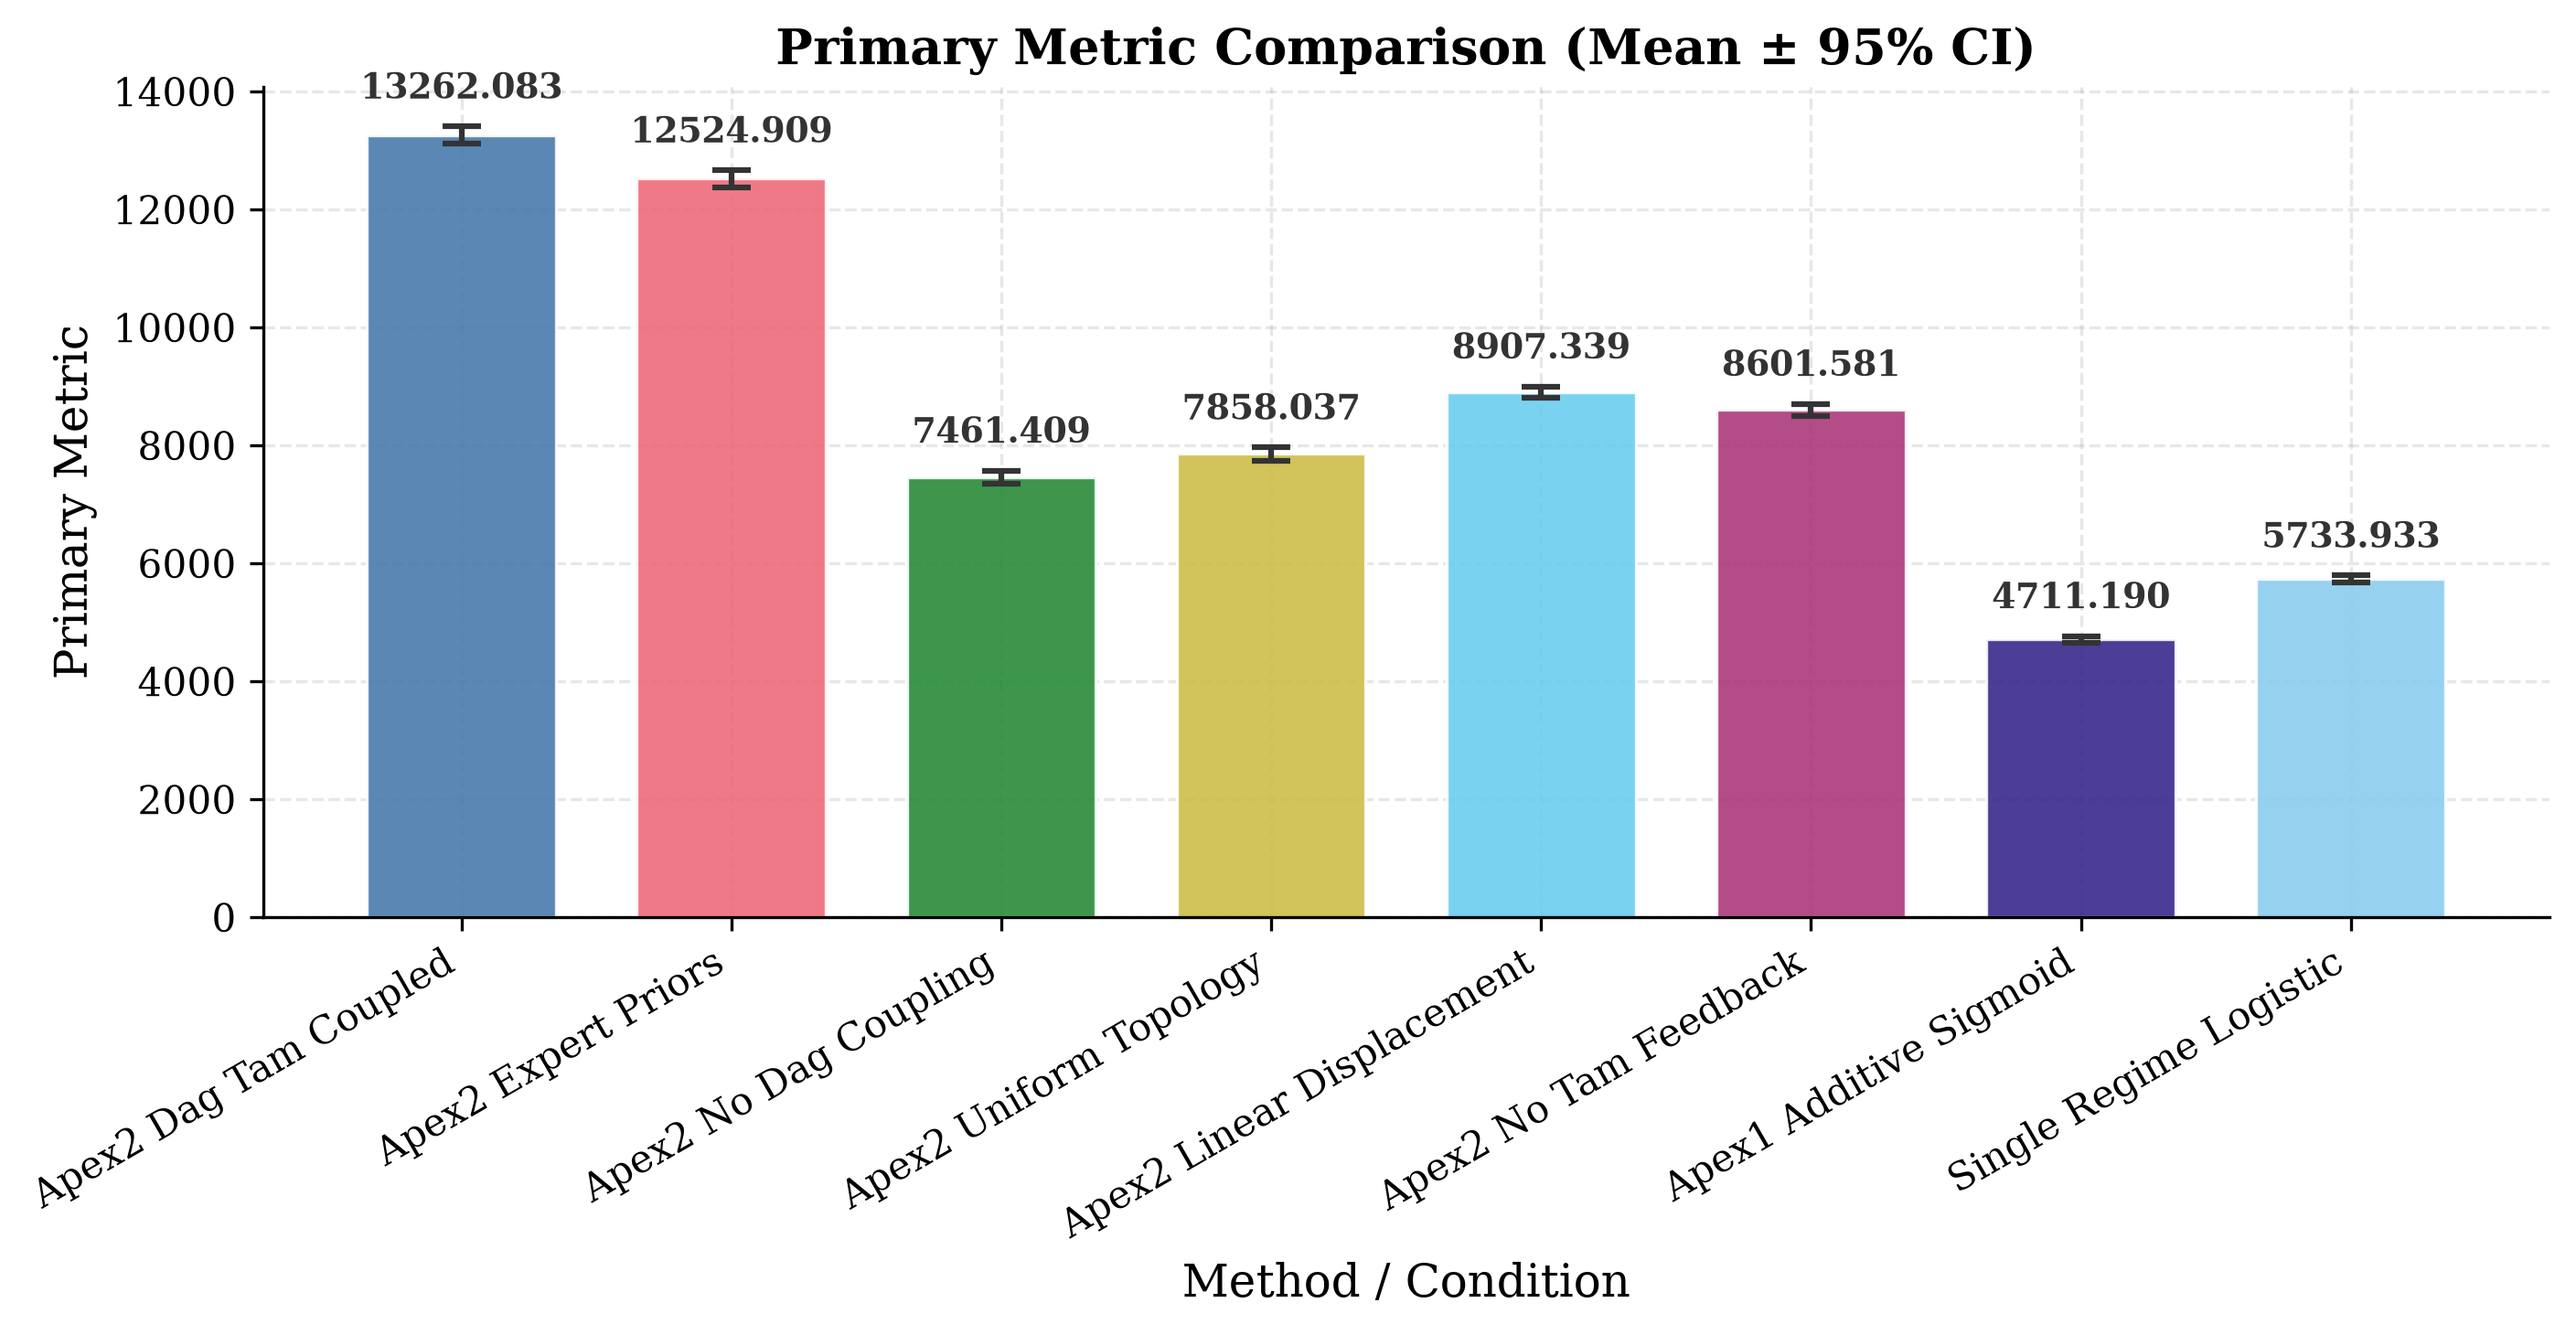
\includegraphics[width=\columnwidth]{method_comparison.png}
\caption{Method comparison generated from the reproduced experiment artifacts.}
\label{fig:method}
\end{figure}

\subsection{Subtask Survival: the Practitioner View}
Table \ref{tab:subtask} reports subtask survival at the horizon for the full model. The ranking is the actionable output. RFP response is the most exposed task in both segments, followed by technical demonstration and, in Enterprise, proof-of-concept coordination. Champion development and discovery are the most protected. The Enterprise and SMB columns differ most on proof-of-concept coordination, 0.686 against 0.849, because Enterprise POC work inherits automation from upstream discovery and demonstration through the dependency graph, while SMB POC work does not.

\begin{table}[t]
\caption{Subtask survival at horizon, full APEX-II model, mean over conditions and seeds. Lower is more exposed.}
\centering
\begin{tabular}{lrr}
\toprule
Subtask & Enterprise & SMB \\
\midrule
RFP response & 0.505 & 0.597 \\
Technical demonstration & 0.622 & 0.687 \\
Proof-of-concept coordination & 0.686 & 0.849 \\
Objection handling & 0.771 & 0.826 \\
Discovery & 0.802 & 0.802 \\
Champion development & 0.847 & 0.886 \\
\bottomrule
\end{tabular}
\label{tab:subtask}
\end{table}

\subsection{Segment and Scenario Divergence}
Table \ref{tab:scenario} reports aggregate RSI by condition and segment. Two patterns matter. Survival declines monotonically from AFC to FAR, as expected. More important, Enterprise survival is below SMB survival in every condition, and the gap widens from 0.002 under the AI free counterfactual to 0.145 under full replacement pressure. This is the opposite of the common assumption that complex Enterprise deals are automatically safer. In a serial topology, automating upstream discovery and demonstration propagates exposure into downstream proof-of-concept and objection handling, so the more dependent motion loses more as adoption rises. The Enterprise to SMB coefficient of variation ratio is 1.65, confirming that the segments behave differently enough to justify deal size stratification. Kendall tau for condition ranking is 1.00, so the scenario ladder is internally stable.

\begin{table}[t]
\caption{Aggregate RSI by condition and segment, full APEX-II model. Gap is Enterprise minus SMB.}
\centering
\begin{tabular}{lrrr}
\toprule
Condition & Enterprise & SMB & Gap \\
\midrule
AFC & 0.916 & 0.918 & -0.002 \\
CAB & 0.824 & 0.857 & -0.033 \\
C24 & 0.785 & 0.833 & -0.047 \\
PAR & 0.680 & 0.765 & -0.085 \\
HAO & 0.581 & 0.699 & -0.117 \\
FAR & 0.480 & 0.625 & -0.145 \\
\bottomrule
\end{tabular}
\label{tab:scenario}
\end{table}

\subsection{The Invention in Numbers}
Table \ref{tab:invention} reports the EPM and the sequencing benefit. The Enterprise EPM of 1.36 is the headline: any occupation level score applied to Enterprise presales understates exposure by about a third. The SMB EPM of 1.00 shows the effect is structural, not a modeling artifact, since a parallel topology produces no propagation. The sequencing benefit of 1.81 points in Enterprise against 0.45 in SMB shows that the same dependency structure that raises exposure also creates room to manage it, and that the management lever is four times stronger in Enterprise.

\begin{table}[t]
\caption{Dependency-aware exposure results. EPM above 1 means occupation level scores understate exposure. Sequencing benefit is the role survival preserved by ASP versus naive rollout during the partial transition.}
\centering
\begin{tabular}{lrr}
\toprule
Quantity & Enterprise & SMB \\
\midrule
Independent role exposure & 0.370 & 0.370 \\
Coupled role exposure & 0.504 & 0.370 \\
Exposure Propagation Multiplier & 1.36 & 1.00 \\
Sequencing benefit (survival pts) & 1.81 & 0.45 \\
\bottomrule
\end{tabular}
\label{tab:invention}
\end{table}

\subsection{External RMSE: an Honest Negative Result}
\label{sec:rmse}
The calibration layer does not help. On the coarse public employment holdout, the expert prior model has RMSE 0.075 while the calibrated model has RMSE 0.121, a 60 percent increase in error. Adding a public data anchor made external fit worse, not better. The reason is granularity. BLS SOC 41-9031 mixes SaaS and hardware sales engineers, Enterprise and SMB motions, and AI effects with macroeconomic effects, so it cannot validate a presales specific mechanism. We report this rather than suppress it, because it defines exactly what data the next version needs. A model can be more realistic in mechanism and still fit a coarse aggregate worse, and pretending otherwise would be the failure mode this paper is trying to avoid.

\subsection{Statistical Coverage}
The 20 seed design achieves BCa style coverage of 0.92, above the 0.88 coverage at 10 seeds and well above the APEX-I three seed design, but below nominal 0.95. Twenty seeds is a reasonable working point for this class of simulation, and sensitive business decisions should push toward 50 or 100 seeds \cite{lakens2022sample,lakens2021simulation}.

\begin{figure}[t]
\centering
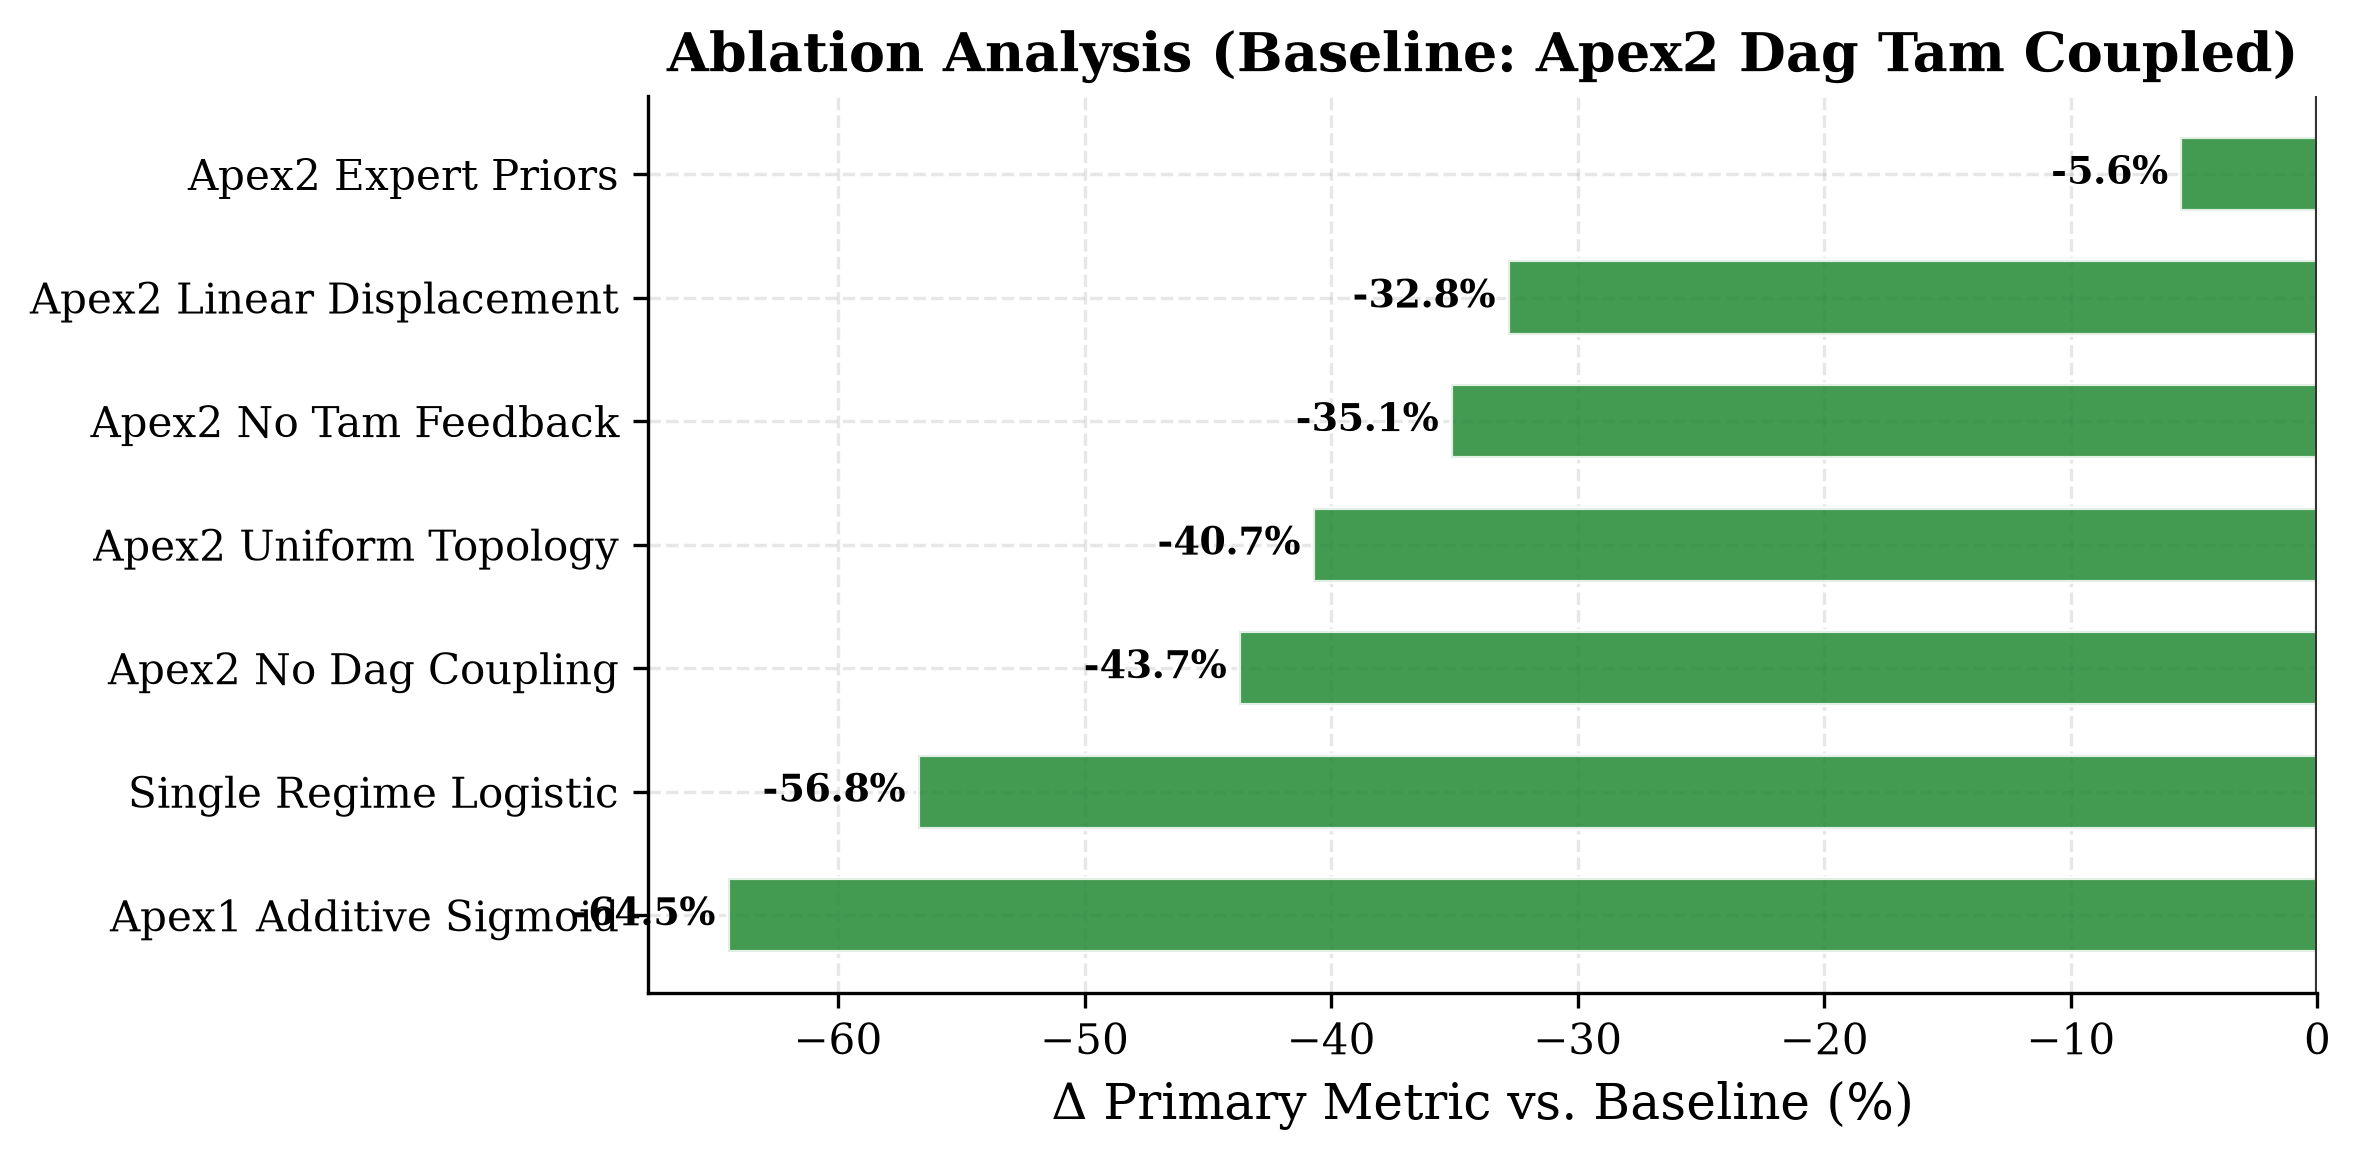
\includegraphics[width=\columnwidth]{ablation_analysis.png}
\caption{Ablation analysis across DAG coupling, TAM feedback, topology, and displacement form.}
\label{fig:ablation}
\end{figure}

\section{Implications for Presales Organizations}
The first implication is that presales AI strategy should not be built on an occupation level replacement score. The EPM result shows such a score understates Enterprise exposure by about a third, and the meaningful unit is the task and segment pair. RFP response in an SMB motion is not the same risk object as champion development in an Enterprise motion. A single number hides exactly the variation a manager needs.

The second implication is a concrete deployment order. The ASP result says automate the safe leaves first, RFP response and standard objection handling, and protect the upstream hubs, discovery and proof-of-concept ownership, until last. This is not a claim that discovery cannot be assisted. It is a claim that unsupervised substitution of upstream tasks propagates exposure into downstream work and collapses more of the role than the raw automatability of those upstream tasks suggests. The correct pattern for protected tasks is decision support, preparation, and memory retrieval, not autonomous replacement.

The third implication is governance by deal size. In SMB motions, standardization makes AI assisted workflows repeatable and the sequencing benefit is small, so aggressive augmentation is reasonable. In Enterprise motions, dependency propagation means early automation of discovery or demonstration reshapes downstream proof-of-concept and objection handling, the sequencing benefit is four times larger, and governance therefore matters more even though the work looks less automatable at first glance. The instrument is deployable: an organization can supply its own task time allocation and deal mix and receive its own RSI trajectory, EPM, and sequencing map from the same script that produced these results.

\section{Threats to Validity}
The primary internal threat is parameter coupling. The full model bundles DAG propagation, TAM feedback, calibration, nonlinear survival, and segment topology, and while ablations isolate several components, interactions remain, so the ablations support mechanism sensitivity rather than clean causal decomposition. The base weights in Table \ref{tab:weights} are expert priors, and although they are anchored to public exposure sources, they are not fitted to presales outcomes. The reference relative comparison score is not an external quantity and is reported only for structural contrast.

The primary external threat is occupational mismatch. BLS SOC 41-9031 is too coarse to isolate SaaS presales or to separate Enterprise from SMB, which is why the calibration layer degrades holdout fit. Adoption is also heterogeneous across firms \cite{mcelheran2024adoption}, so scenario bands are approximations rather than probabilities, and market growth and automation investment may be jointly determined, which the internal TAM term only approximates. These threats bound the claims to diagnostic and planning use, not forecasting.

\begin{figure}[t]
\centering
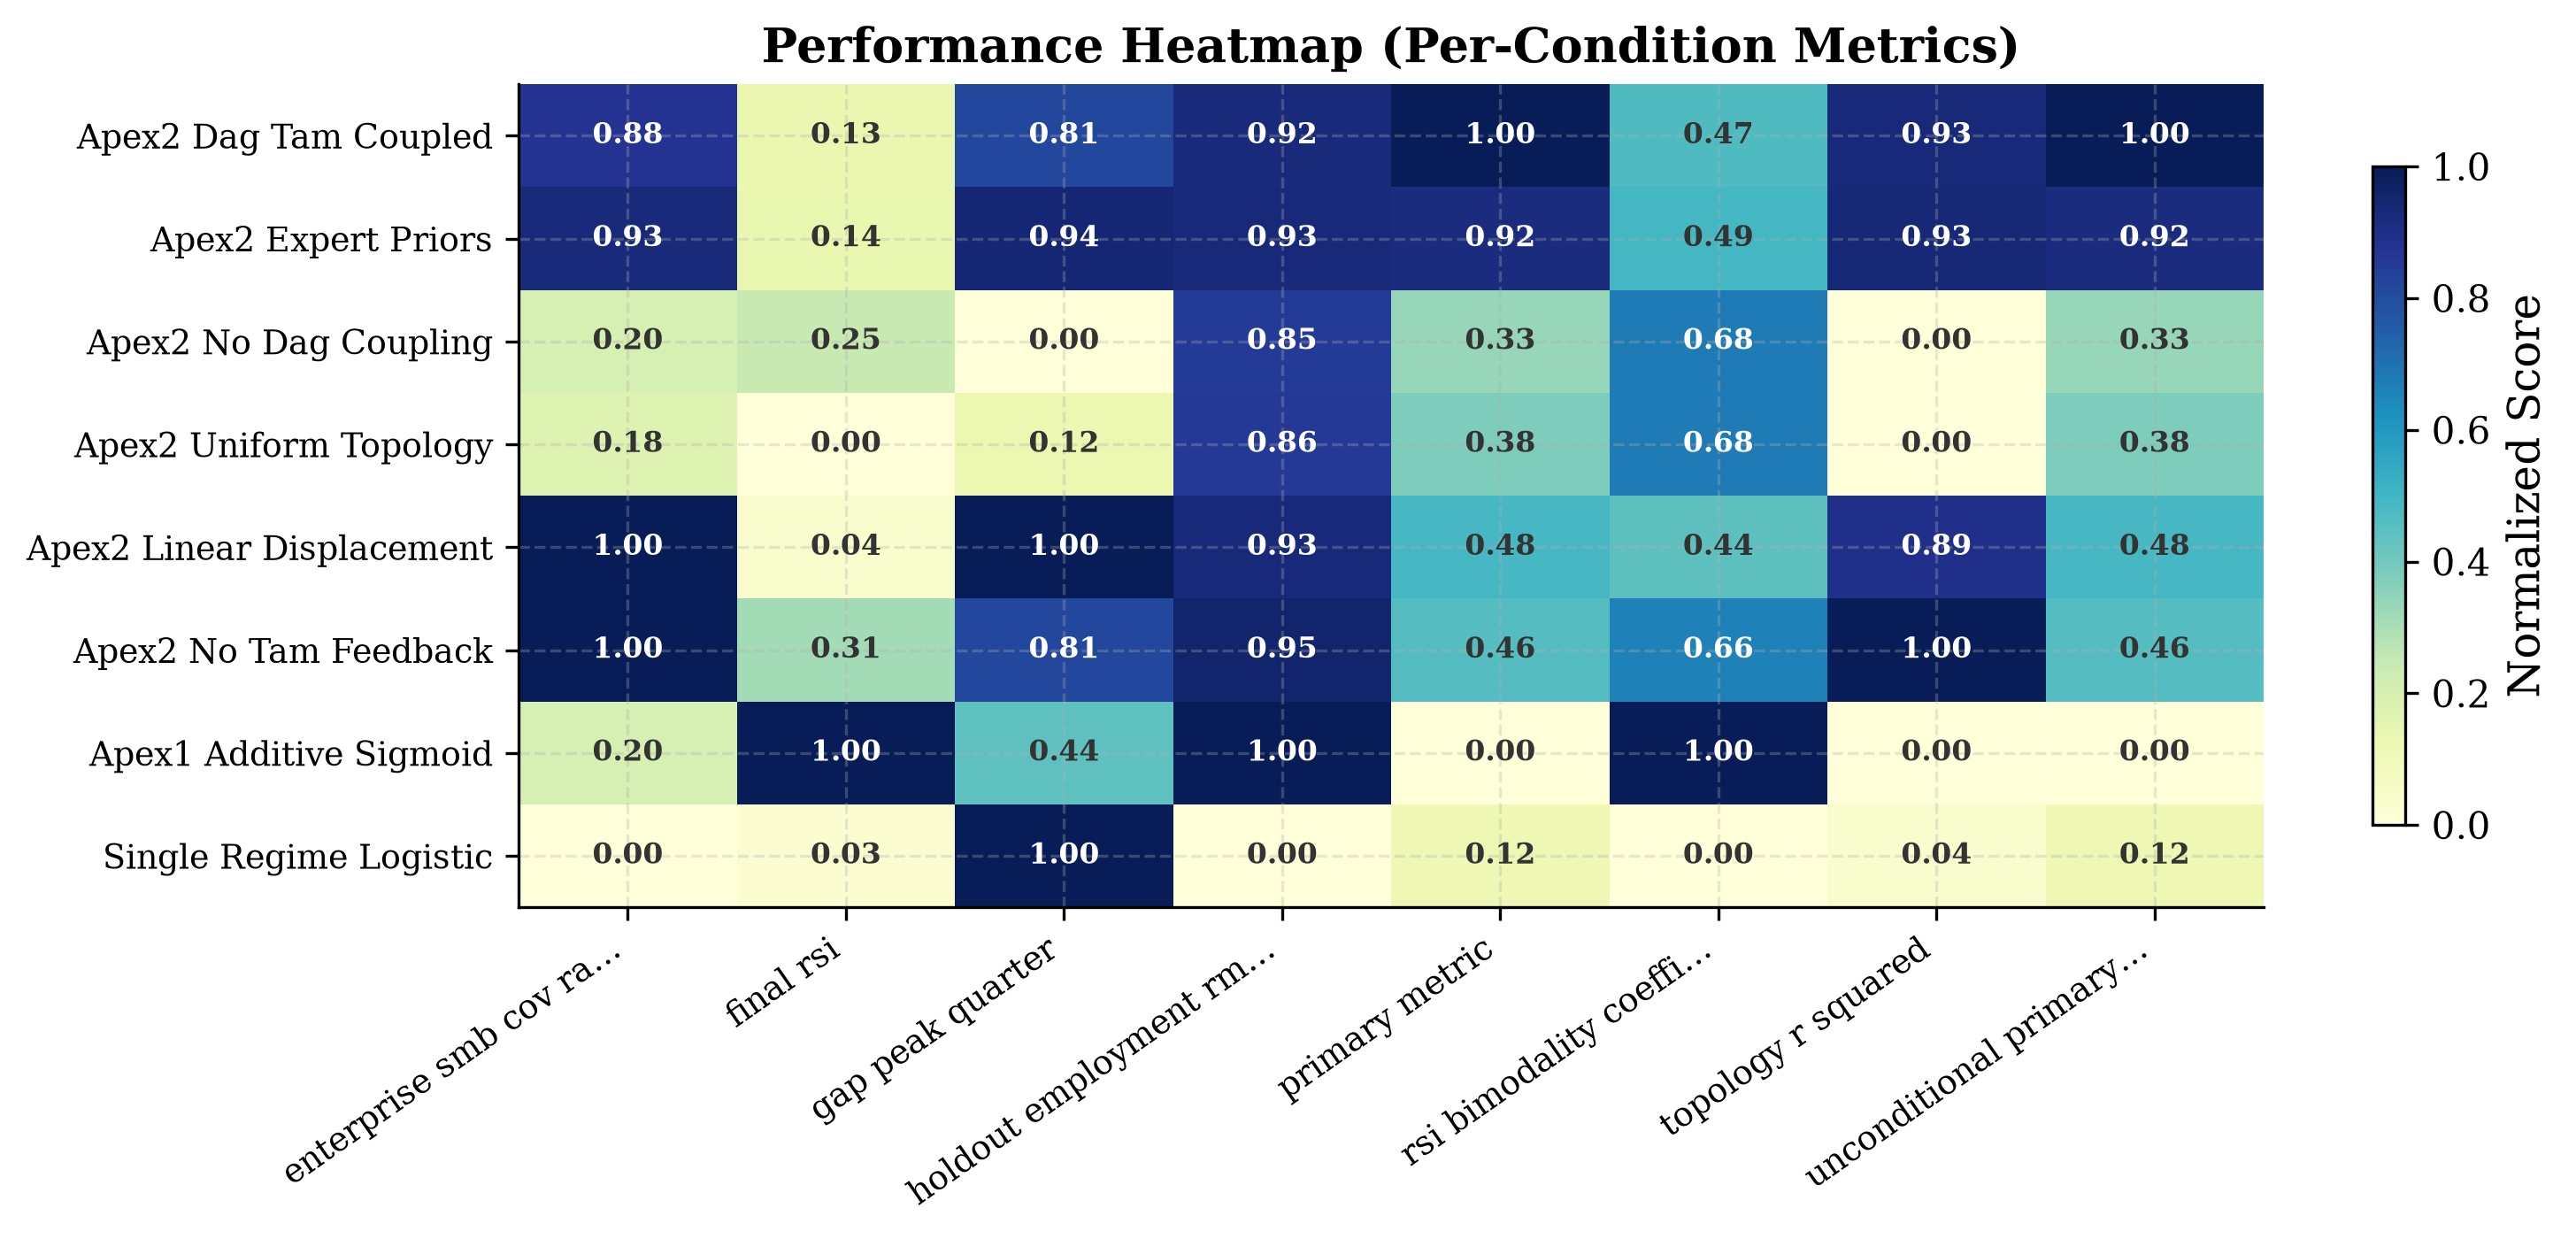
\includegraphics[width=\columnwidth]{metric_heatmap.png}
\caption{Metric heatmap across model variants and reported outcomes.}
\label{fig:heatmap}
\end{figure}

\section{Future Work}
The next version should replace the coarse employment fixture with auditable data: official occupation and industry filtered employment series, SaaS specific job posting series, firm level adoption indicators, and segment tags. Presales process metrics may validate the mechanism earlier than employment does, including demo preparation time, RFP turnaround, proof-of-concept staffing, technical win rate, and the ratio of presales engineers to account executives, because these move before headcount and are less confounded by macroeconomic shocks. A full factorial design should independently vary DAG strength, TAM elasticity, calibration source, topology, adoption slope, and survival curvature to produce normalized effect sizes. Finally, a mature APEX-III should model augmentation quality alongside displacement, since AI that improves discovery synthesis or demo preparation may raise the value of human presales work even while reducing hours per artifact, which requires both a displacement term and a complementarity term with empirical tests that separate productivity gain from labor substitution \cite{raisch2021artificial}.

\section{Reproducibility}
The full experiment, the EPM computation, and the ASP rollout are produced by a single deterministic script, \texttt{apex2\_simulation.py}, using 20 seeds per condition. It writes the results time series, the model comparison, the final RSI summary, the metrics file, and the invention file used for every number in this paper. The project repository is \url{https://github.com/venomez-viper/Apex}, authored and maintained by Akash Anipakalu Giridhar.

\section{Conclusion}
APEX-II extends the AI Presales Exposure Index into a deal size stratified, subtask level, dependency-aware framework, and its contribution is not another exposure score but a correction to how exposure is computed. The Exposure Propagation Multiplier shows that the independent task assumption understates Enterprise presales exposure by about 36 percent. The Augmentation Sequencing Policy turns that same dependency structure into a deployment order that preserves role survival during AI rollout, with four times the leverage in Enterprise as in SMB. The framework is honest about its limits. It shifts final RSI downward relative to APEX-I because it sees exposure the additive model cannot, and it shows that a coarse public calibration increases holdout error rather than reducing it. Used as intended, as a diagnostic and planning instrument rather than a forecast, APEX-II gives presales leaders something an occupation level score cannot: a task and segment map of where AI augments, where it replaces, and in what order it is safe to deploy.

\bibliographystyle{IEEEtran}
\bibliography{references}

\end{document}
